
\documentclass[10pt]{article}

\parindent=0pt

\usepackage{fullpage}

\frenchspacing

\usepackage{microtype}

\usepackage[english,dutch]{babel}

\usepackage{graphicx}

\usepackage{listings}
\usepackage{caption}

\lstset{language=C++, showstringspaces=false, basicstyle=\small,
  numbers=left, numberstyle=\tiny, numberfirstline=false, breaklines=true,
  stepnumber=1, tabsize=8, 
  commentstyle=\ttfamily, identifierstyle=\ttfamily,
  stringstyle=\itshape}

\usepackage[setpagesize=false,colorlinks=true,linkcolor=red,urlcolor=blue,pdftitle={Kunstmatige Intelligentie bij Tetris},pdfauthor={Alex Keizer}]{hyperref}

\author{Bram Honig \and Alex Keizer}
\title{Kunstmatige Intelligentie bij Tetris}

\begin{document}

\selectlanguage{dutch}

\maketitle

\section{Inleiding} 
Tetris staat voornamelijk bekend als een spelletje waar je een goed reactievermogen voor moet hebben. Toch zorgen de vele mogelijke manieren om een stuk te plaatsen het feit dat je niet weet welke stukken nog gaan komen ervoor dat het zeker niet recht toe recht aan duidelijk is wat de beste zet op een gegeven moment is. In onze zoektocht zullen wij ons slechts beperken tot het stuk wat we op een gegeven moment ktijgen en niet nog zetten vooruit gaan denken.

Waarschijnlijk kennen de meesten de regels van Tetris wel, maar voor de volledigheid zullen we ze nog noemen. Elke zet krijg je een stuk, waar de speler moet bepalen op welke plek en met welke rotatie we het laten vallen. Dit mag, in onze variatie, tijdens het vallen niet veranderd worden. Als een rij compleet vol zit zal deze worden weggehaald en de vakjes erboven zullen een rij naar beneden vallen. Het spel is voorbij wanneer een stuk niet meer op het bord past.

\section{Uitleg probleem}\label{probleem}

Elke ``beurt'' krijgen we een (willekeurig) stuk, onze zet bestaat dan vervolgens uit de kolom waar we dat stuk laten vallen en met welke rotatie we dat doen. In onze variatie hebben we dus geen kennis over welk stuk gaat volgen. Aangezien er aanzienlijk wat mogelijkheden zijn is het erg lastig om te bepalen wat de optimaalste zet is. Zelfs als een preciese reeks stukken gegeven wordt is het een NP-hard probleem om de beste zetten te vinden. \cite{nphard} (zie sectie \ref{relevant})

\section{Relevant werk}\label{relevant}

In eerder onderzoek is aangetoond dat het bepalen van de beste zetten een NP-hard probleem\cite{nphard} is---dit geldt zowel als je geplaatste stukken of weggehaalde rijen als score gebruikt. Dit houdt in dat als er een oplossing wordt aangeboden deze heel makkelijk te verifieren is, echter om een (optimale) oplossing te vinden kost dat op zijn minst polynomiale tijd. Als het probleem complexer wordt, wordt de tijd die het kost om een oplossing te vinden extreem groeit.

Om deze reden is er ook onderzoek gedaan naar hoe goed een heuristisch algoritme tetris kan spelen, waarbij een zet a.d.v. een aantal kenmerken en co\"{e}ficenten voor die kenmerken worden beoordeeld. Bij het onderzoek uit 2015 ``An Evolutionary Approach to Tetris'' \cite{genetic} werden 12 kenmerken gebruikt waar de evualatie functie zich op baseerde. Drie hiervan gebruiken wij ook: (zie sectie \ref{aanpak} voor uitleg van deze punten)
\begin{itemize}
\item Hoogste rij
\item Weggehaalde rijen
\item Gaten
\item Hoogte verschil
\end{itemize}

Om het gewicht van elk kenmerk te bepalen werd gebruik gemaakt van een genetisch algoritme. Een van de conclusies was dat er veel locale optima waren waar het algoritme niet kon ontsnappen. Verder werd geconstateerd dat het bepalen van de optimale gewichten erg veel tijd in beslag neemt---een van de tests heeft 3 maanden gedraaid.


\section{Aanpak}\label{aanpak}
Als eerste poging is er een Monte Carlo algoritme ge\"{i}mplementeerd. Bij elke beurt wordt elke mogelijke zet een vast aantal willekeurige potjes gespeeld. De zet waarbij in al die spelletjes het meeste stukken werden gespeeld wordt gekozen als de beste zet.

Willekeurig spelen is niet erg effici\"{e}nt, dus hebben we ook een ``slim'' algoritme. Zoals gezegd in sectie \ref{probleem} wordt een speelboom al snel erg groot, wij hebben ons dus beperkt tot alle mogelijkheden met het huidige stuk. Elk van deze mogelijkheden wordt ge\"{e}valueerd aan de hand van de volgende punten:
\begin{itemize}

\item \textbf{Hoogste Rij} De hoogste rij met bezette vakjes (in het kwadraat)

\item \textbf{Hoogste Legen} Aantal lege vakjes in de hoogst bezette rij

\item \textbf{Weggehaalde rijen} Aantal rijen dat tijden het spel weg zijn gehaald, omdat ze compleet waren

\item \textbf{Gaten} Lege vakjes met erboven (in dezelfde kolom) een niet-leeg vakje

\item \textbf{Hoogte Verschil} Het hoogteverschil tussen opeenvolgende rijen

\end{itemize}
Hoe hoger de stapel wordt, hoe erger het is als hij verder stijgt (je komt immers telkens dichter bij het einde). We hebben dus niet direct het nummer van de hoogste rij gepakt, maar het kwadraat daarvan als meetpunt. Elk van deze punten wordt vervolgens met een co\"effici\"ent vermenigvuldigd en bij elkaar opgeteld, dit is de uiteindelijke score voor dat bord (en de zet die tot dat bord heeft geleid). Verder wordt natuurlijk weer de zet met de hoogste score gedaan.

\section{Implementatie}

Wij hebben in C++ geprogrammeerd. De basis voor de slimme-, en Monte Carlo speler is hetzelfde. Met \verb+possibilities (piece)+ wordt bepaald hoeveel zetten er mogelijk zijn, elke zet wordt vervolgens gescoord door ofwel \verb+evaluatemove(piece, themove)+ (slim), ofwel \verb+evaluateMonteCarlo(piece, themove)+ (Monte Carlo).

\verb+evaluatemove(piece, themove)+ maakt als eerste een kopie van het \verb+Tetris+ object, voert de zet uit en bepaalt de eerder gegeven kenmerken---hoogste rij, hoogste legen, weggehaalde rijen, gaten en hoogte verschil---deze worden vermenigvuldigd met de bijbehorende co\"{e}fficienten (vastgelegd in het \verb+TetrisScore+ struct gegeven in de constructor van \verb+Tetris+) en opgeteld. Deze laatste waarde is wat gereturned wordt als score.
\verb+evaluatemontecarlo(piece, themove)+ maakt eveneenst eerste een kopie en voert de zet uit. Verder worden er een vast aantal ($monte\_loop$) keer nog een kopie van de staat na de zet gemaakt, een willekeurige potje gespeeld met \verb+playrandomgame( )+ en de uiteindelijk verkregen $piececount$, het aantal gespeelde stukken, van alle potjes opgeteld. Deze totaalscore wordt gereturned.

Welke van de evaluatiefuncties gebruikt wordt, wordt bepaald door de $EvalName$ die aan \texttt{playgame(EvalName eval)} gegeven wordt.

\section{Experimenten}

We hebben een aantal experimenten uitgevoerd, voornamelijk hoe beide spelers reageren op de bepalende parameters ($monte\_loop$ en de co\"efici\"enten). Daarnaast hebben we van beide spelers bekeken hoe ze reageren op verschillende bord groottes.

\subsection{Monte Carlo}
Ten eerste hebben wij bij de Monte Carlo speler het aantal willekeurige potjes---$monte\_loop$---gevarieerd. Wij hebben voor elke variatie 1000 keer gespeeld, waarbij we bijhouden hoe lang dit duurde en hoe veel stukken gespeeld zijn. Deze tests zijn gedaan op een $15 \times 20$ bord. Absoluut is deze tijd sterk afhankelijk van o.a. de gebruikte hardware en niet zo interessant, maar de stijging geeft wel degelijk informatie. De tijd uitgezet tegenover $monte\_loop$ is bijna lineair (zie Figuur \ref{fig:monte_score}). Het meeste tijd zal worden gespendeerd aan \verb+playrandomgame( )+, die in \'e\'en spel $\#zetten \times monte\_loop$ keer wordt aangeroepen. Als $monte\_loop$ groter wordt, zal het algoritme iets beter werken en dus meer zetten doen. Echter is $monte_loop$ vaak significant groter, waardoor het alsnog bijna lineair is. De behaalde score tegenover $monte\_loop$ is exponenti\"el dalend. Door de willekeurige aard van het Monte Carlo algoritme is dit niet heel vreemd, een $11^e$ poging heeft redelijk kans een betere weg te vinden dan de eerste $10$. Een $101^{ste}$ poging is daarentgen veel minder waarschijnlijk beter dan de eerdere $100$.
Hoe groter $monte\_loop$ wordt, hoe minder effici\"ent het algoritme wordt. Elke stijging van $monte_loop$ zorgt voor een (iets) grotere stijging van de gespendeerde tijd, meer steeds minder stijging van behaalde score.

\begin{figure}
\begin{center}
\includegraphics{carlo.eps}
\caption{Behaalde score en tijd uitgezet tegen $monte\_loop$}\label{fig:monte_score}

\end{center}
\end{figure}



\subsection{Slimme Speler}
Voor het bepalen van de co\"efici\"enten hebben we een aantal logisch lijkende beginwaarden gekozen en hebben we (handmatig) wat gevarieerd. In het begin hebben we getest met 1000 potjes Tetris per variatie, maar hebben ons uiteindelijk tot 100 iteraties vanwege de lange tijd dat een potje duurde. Helaas werd de variatie erg groot---2 potjes met precies eenzelfde configuratie, maar andere seed, hadden een score van $106$ en $60.000$ zetten---en kost het verkrijgen van een enigszins representatief gemiddelde erg veel iteraties en dus tijd. We hebben ons daarom vastgelegd op de configuratie in Figuur \ref{fig:smart_coef}, in de kennis dat er waarschijnlijk een veel optimalere configuratie is.

Deze waardes hebben we wel nog verder getest. We hebben voor elk kenmerk besloten om de andere constant te houden (zodat we maar $5n$ en geen $n^5$ tests hoeven draaien). Daarbij vermenigvuldigen we de specifieke co\"effici\"ent met de getallen $\{0.1, 0.2, 0.5, 0.8, 1, 2.5, 5, 7.5, 10 \}$ en spelen met elk 500 potjes. Het bord kiezen we weer maximaal, $15 \times 20$.

\begin{figure}
\begin{center}
\begin{tabular}{l|c}
	Hoogste Rij		& $-10$ \\ \hline
	Hoogste Legen		& $50$ \\ \hline
	Weggehaalde Rijen	& $150$ \\ \hline
	Gaten			& $-200$ \\ \hline
	Hoogte Verschil		& $-10$ \\
\end{tabular}
\end{center}
\caption{Co\"{e}fici\"{e}nten voor de slimme speler}\label{fig:smart_coef}
\end{figure}

\begin{figure}
	\begin{center}
	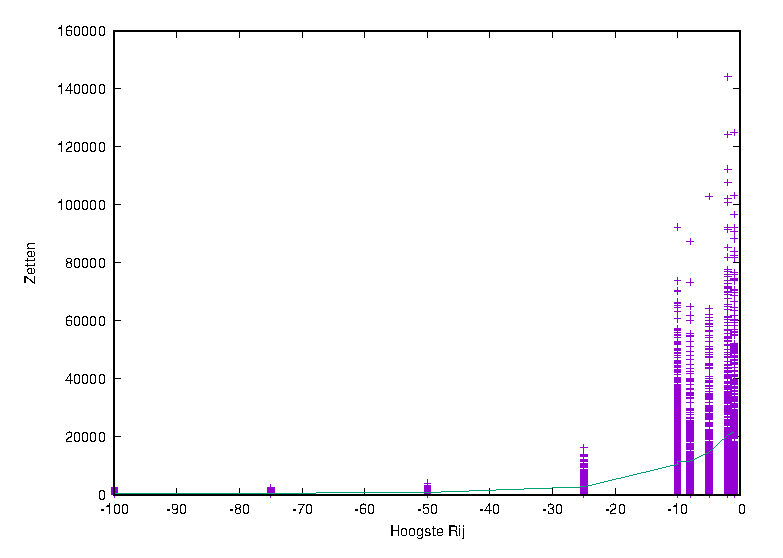
\includegraphics[height="5cm"]{div1.eps}
	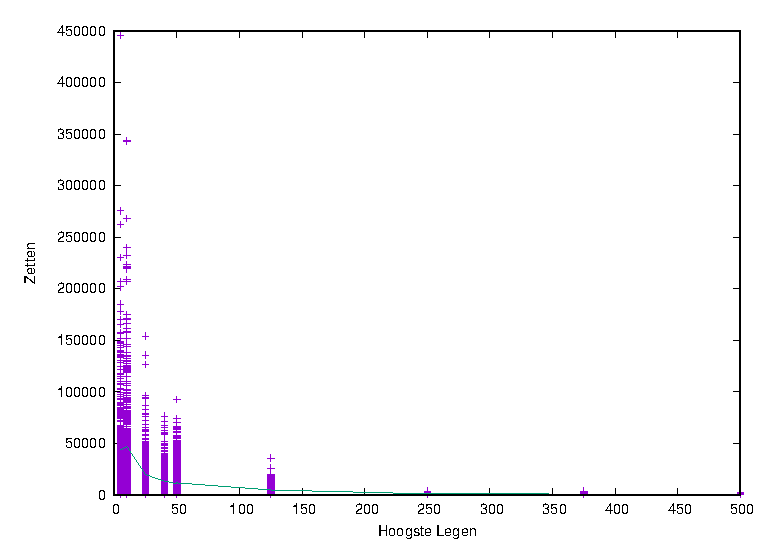
\includegraphics[height="5cm"]{div2.eps}
	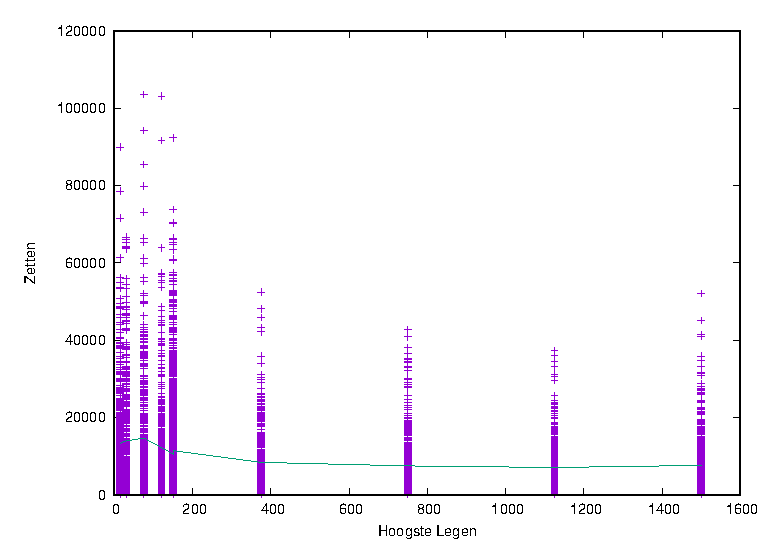
\includegraphics[height="5cm"]{div3.eps}
	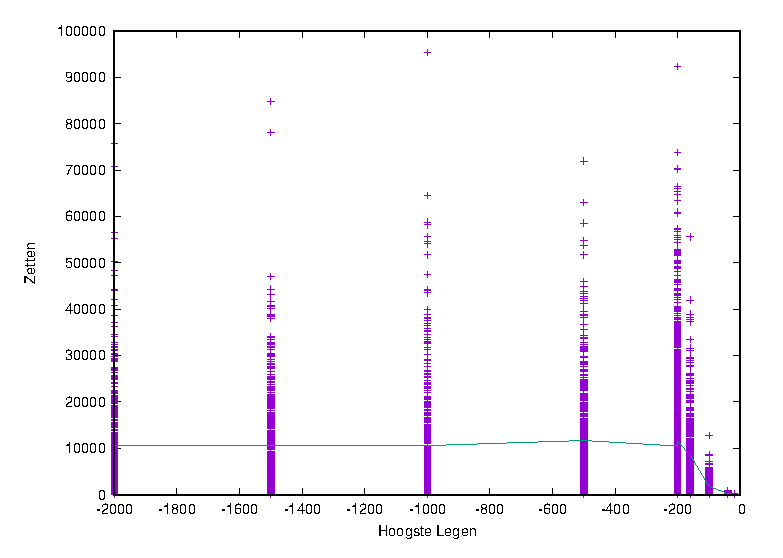
\includegraphics[height="5cm"]{div4.eps}
	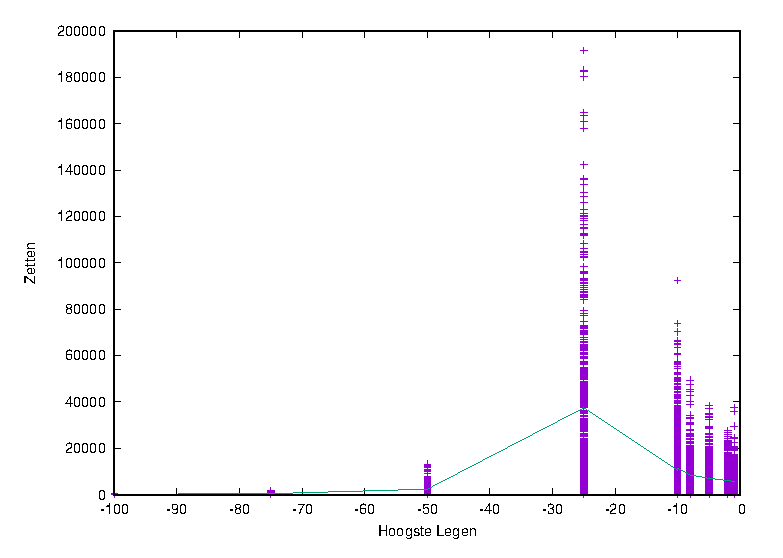
\includegraphics[height="5cm"]{div5.eps}
\end{center}
\end{figure}

\subsection{Bord Groottes}
We hebben eveneens beide spelers getest op verschillende bord groottes. Voor Monte Carlo hebben we $monte\_loop = 500$ gebruikt, voor de slimme speler hebben we de co\"effici\"enten uit Figuur \ref{fig:smart_coef} gebruikt. De score is bepaald als gemiddelde van 500 gespeelde potjes, daarnaast hebben we de standaardfout van dat gemiddelde bepaald. De resultaten staan in Figuur~\ref{fig:monte_bord} en Figuur~\ref{fig:smart_bord}. Voor Monte Carlo valt op dat het vooral van extra lengte profiteert, maar extra breedte niet zo goed kan benutten. In principe is dit effect---meer lengte is beter dan meer breedte---verklaarbaar door het feit dat extra breedte, naast het geven van extra ruimte, ook ervoor zorgt dat het weghalen van rijen lastiger wordt. Verder is er maar ruwweg een factor $~5$ verschil tussen de hoogste en laagste scores, wat komt doordat we bij het bepalen van de co\"effici\"enten alleen met een $15 \times 20$ bord hebben getest.

De slimme speler vertoont juist het tegenovergestelde---extra breedte zorgt voor significant betere prestaties dan extra lengte. Dit is lastiger te verklaren, maar schuilt waarschijnlijk in het feit dat onze Weggehaalde Rijen met $150$ zwaar meeweegt of dat het algoritme door de Hoogste Rij factor de lengte sowieso vermijdt. Op de kleinst geteste breedte ($w=4$) doet Monte Carlo het zelfs consistent beter. De hoogste en laagste scores verschillen hier met een factor $750$. Verder zien we hier weer de gigantische inconsistentie tussen de scores terugkomen in de standaardfout.

\begin{figure}
$$\begin{array}{l||c|c|c|c|c}
	    & 4 			& 8 			   & 12 			& 16 			 & 20 \\ 
	\hline\hline
	8  & 18.2 (\pm 11.5) 	& 24.3 (\pm 11.7) & 25.8 (\pm 11.1)  & 27.3 (\pm 9.6)  & 28.5 (\pm 7.8) \\
	12 & 41.7 (\pm 22.9) & 61.6 (\pm 28)    & 62 (\pm 23.5)     & 60.6 (\pm 18.2) & 59.1 (\pm 15.1)  \\
	15 & 59.7 (\pm 30.2) & 91.6 (\pm 41.8) & 86.7 (\pm 29)     & 81.4 (\pm 22.4) & 77.5 (\pm 16.4) \\
\end{array}$$
\caption{Gemiddeld behaalde zetten (en standaardfout) van Monte Carlo op verschillende bordgroottes, bepaald door 500 tetris potjes met $monte\_loop=500$}\label{fig:monte_bord}
\end{figure}

\begin{figure}
$$\begin{array}{l||c|c|c|c|c}
	    & 4 			& 8 			   & 12 			& 16 			 & 20 \\ 
	\hline\hline
	8  & 14 (\pm 8) 	& 25 (\pm 15) & 46 (\pm 30)  & 81 (\pm 63)  & 148 (\pm 138) \\
	12 & 26 (\pm 16) & 67 (\pm 44)    & 184 (\pm 150)     & 673 (\pm 609) & 2495 (\pm 2475)  \\
	15 & 34 (\pm 20) & 106 (\pm 71) & 345 (\pm 283)     & 1745 (\pm 1688) & 10844 (\pm 9924) \\
\end{array}$$
\caption{Gemiddeld behaalde zetten (en standaardfout) van de slimme speler op verschillende bordgroottes, bepaald door 500 tetris potjes met co\"effici\"enten van Figuur \ref{fig:smart_coef}}\label{fig:smart_bord}
\end{figure}

\section{Conclusie}

Het Monte Carlo algoritme is een aardige manier om snel een bot te maken, maar de scores zijn niet heel goed. Verder is het algoritme niet bijster effici\"ent en stijgen de kosten (iets meer dan) lineair voor exponenti\"el dalende toenames in score, waardoor het algoritme alleen maar minder effici\"ent wordt.

Voor een slimmer algoritme is de keuze en optimalisatie van co\"effici\"enten minstens zo belangrijk als de kenmerken zelf. Helaas kost het bepalen van een representatief gemiddelde score van een configuratie veel test potjes en dus veel tijd. Daarnaast is het belangrijk om te overwegen of het programma op alle bord groottes goed moet functioneren, of dat er voor een bepaalde grootte kan worden geoptimaliseerd---zoals wij niet compleet bewust hebben gedaan.

Verdere verbeteringen zouden kunnen liggen in het toevoegen van meer kenmerken waarop een zet wordt beoordeeld, maar meer winst valt waarschijnlijk te halen door betere optimalisatie van de co\"efici\"enten. 

\begin{thebibliography}{XX}

\bibitem{nphard}
Erik D. Demaine, Susan Hohenberger and David Liben-Nowell, \\
Tetris is Hard, Even to Approximate. \\
In Proceedings of the 9th International Computing and Combinatorics Conference (COCOON 2003) (2003).

\bibitem{genetic}
Niko B\"{o}hm Gabriella K\'{o}kai Stefan Mandl, \\
An Evolutionary Approach to Tetris \\
MIC2005: The Sixth Metaheuristics International Conference \\
\url{https://www2.informatik.uni-erlangen.de/EN/publication/download/mic.pdf}

\end{thebibliography}

\section*{Appendix: Code}

Er is gebruik gemaakt van de \href{http://www.liacs.leidenuniv.nl/~kosterswa/AI/iets.cc}{\underline{skeletcode}} die te vinden is via
de website van het college.
De code van het programma is als volgt:

\smallskip

\lstinputlisting[language=C++]{diff.cc}

\end{document}
